% ==============================================================================
\section{Introduction}
\label{sec:intro}
% ==============================================================================

In modern High-Performance Computing (HPC) systems, Input/Output (I/O) throughput has become as 
critical to overall efficiency as computational capability itself. As supercomputing architectures 
advance toward and beyond the exascale threshold, computational throughput has increased exponentially. 
However, persistent storage bandwidth has lagged behind, widening the compute-to-I/O performance gap. 
For instance, Figure~\ref{fig:io_per_flop} shows how the ratio between I/O bandwidth and compute power 
has evolved over the past two decades for the machines listed in the TOP500~\cite{top500} and IO500~\cite{io500list} 
rankings. Since 2000, the I/O bandwidth available per unit of compute has dropped by roughly $50\times$, from 312 GB/s 
per PFlop/s on ASCI Red down to 6.0 GB/s per PFlop/s on Frontier, with only a modest recovery on the more recent Aurora system. 

Therefore, while modern processors achieve multi-petaflop or exaflop performance, parallel file systems typically deliver only 
hundreds of gigabytes to a few terabytes per second in aggregate write bandwidth. This growing imbalance creates a severe bottleneck: high-performance 
computing tasks spend a non-negligible fraction of their allocated runtime waiting for data transfers to complete.

% Implemented the figure of ratio between compute \& IO

\begin{figure}[h]
  \centering
  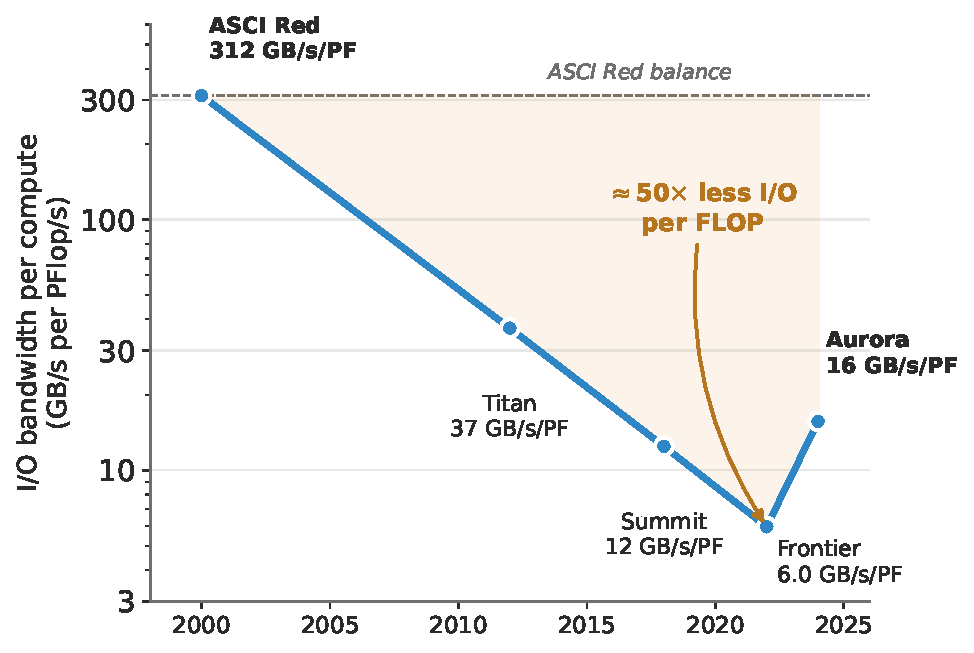
\includegraphics[width=0.55\textwidth]{figures/io_per_flop.pdf}
  \caption{Compute-to-I/O performance gap in Top500 supercomputers (2000--2025). The ratio of storage bandwidth per unit of compute 
  has degraded by more than an order of magnitude.}
  \label{fig:io_per_flop}
\end{figure}

Large-scale scientific simulations generate massive volumes of data requiring efficient parallel management. On shared Parallel File Systems (PFS), 
thousands of concurrent processes must coordinate access to shared storage arrays while contending for network link bandwidth and storage controller 
resources. An example of an application with strong I/O pressure is Gysela, a 5D gyrokinetic simulation code developed by CEA (\textit{Commissariat à 
l'Énergie Atomique et aux Énergies Alternatives}) for nuclear fusion research. Gysela models plasma turbulence in magnetic confinement devices (tokamaks) 
by solving the 5D Vlasov-Poisson system \cite{grandgirard2006gysela}.

Because Gysela executes across hundreds to thousands of computing nodes over extended periods (days to weeks), it relies on periodic checkpointing for fault 
tolerance and job restartability. The checkpointing procedure is synchronous: all parallel processes pause numerical integration, aggregate their local state 
vectors, and flush the 5D distribution function to persistent storage. A single checkpoint operation can generate terabytes of data, putting strong pressure on
the storage system and interfering with the other applications that share it. Moreover, during this phase, compute resources remain idle, and in shared production 
environments, the write times exhibit high variability—sometimes exceeding median write durations by a factor of up to 30 \cite{trochon2025checkpointing}.—due to 
concurrent I/O contention from uncoordinated tenant jobs.

Optimizing I/O performance requires a coordinated approach across two complementary layers: the PFS configuration, which involves adjusting low-level layout
parameters, such as striping count (number of storage targets) and stripe size, and high-level I/O strategies, which determine how application data structures 
are mapped, aggregated, and formatted before being dispatched to storage (e.g., Single Shared File, Subfiling, or File Per Process). In this work, we explore
both layers: we conduct a tuning study over several parameters that affect the I/O behaviour of Gysela's checkpoint procedure. Our objective is to determine 
which configuration maximizes I/O performance, and to characterize how each parameter contributes to it. 

To enable rapid, reproducible experimentation without incurring the massive computational cost of full plasma physics simulations, we employ gys\_io, a dedicated 
mini-application that faithfully reproduces Gysela's 5D checkpoint I/O access pattern\cite{gysela_miniapp_io}.

% --- INSTITUTIONAL & PROJECT CONTEXT (integrated) ---
This work was carried out within the \textsc{TADaaM} research team (\textit{Topology-Aware system-scale Data management for high-performance computing}) at 
the Inria Centre at the University of Bordeaux. TADaaM designs system software and data-management layers that bridge the gap between application-level 
requirements and complex hardware topologies in HPC environments. The study is framed within the \textbf{NumPex} program, the French national initiative building 
the software ecosystem for exascale supercomputing, and more specifically within the \textbf{Exa-DOST} work package, which targets advanced I/O optimisation 
strategies and dynamic data-management middlewares for extreme-scale applications. Collaborative ties between Inria TADaaM and CEA motivate the choice of Gysela 
as the target application: joint efforts between the two institutions aim to prepare Gysela's I/O substrate for upcoming European exascale machines, including 
Alice Recoque in France.

The remainder of this report is organized as follows. Section~\ref{sec:context} presents the institutional and project context of this work. 
Section~\ref{sec:background} reviews how parallel file systems distribute data across storage targets and describes the three parallel write strategies 
we evaluate, together with the software stack used to run the experiments. Section~\ref{sec:setup} details the experimental setup: the clusters and their 
storage systems, the benchmark workload, and the range of parameters explored. \todoitem{extend this roadmap once the results and conclusion sections exist}

